%%%% début de la page
\teteSndCorp

%%%% titre
\nomPrenomClasse
\titreTP{Séparer et identifier des espèces chimiques}


%%%% objectifs
\begin{objectifs}
  \item Réaliser et analyser une Chromatographie sur Couche Mince.
\end{objectifs}


%%%% evaluation
\begin{tableauCompetences}
  VAL & Comparer des valeurs mesurées avec des valeurs de références.
\end{tableauCompetences}



%%%% contexte
\begin{contexte}
  En Europe, les colorants alimentaires sont désignés par un préfixe E suivi d'un numéro.
  Ces colorants se retrouvent dans de nombreux produits.
  
  On cherche à déterminer les colorants présent dans des M\&M's à l'aide d'une \important{Chromatographie sur Couche Mince (CCM).}
\end{contexte}


%%%% document
\begin{doc}{Chromatographie sur Couche Mince (CCM)}{doc:TP4_CCM}
  \begin{wrapfigure}{l}{0.45\linewidth}
    \centering
    \vspace*{-16pt}
    \image{0.9}{images/chimie/CCM/CCM.png} \\
    \legende{Schéma expérimental d'une CCM.}
  \end{wrapfigure}

  La \important{chromatographie sur couche mince (CCM)} permet de séparer et d'identifier des espèces chimiques dans un mélange.

  Le principe est le suivant : on dépose les espèces à identifier sur une plaque, appelée \important{phase stationnaire.} On fait tremper une partie de la plaque dans un liquide appelé \important{éluant}.
  
  Par capillarité, l'éluant va monter le long de la plaque et les espèces déposées sur la plaque vont être poussées par l'éluant pendant sa montée.
  
  En fonction de leurs propriétés, les espèces chimiques seront poussées plus ou moins haut sur la plaque, ce qui permettra de les identifier.
  La fiche ainsi formée est appelée un \important{chromatogramme}.
\end{doc}

%%%%
\begin{doc}{Réalisation d'une CCM}{doc:TP4_protocole_CCM}
  \begin{multicols}{3}
    \begin{center}
      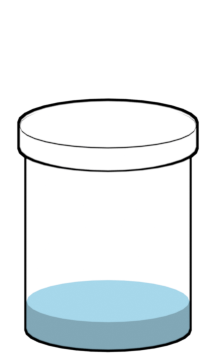
\includegraphics[height=0.2\textheight]{images/chimie/CCM/CCM_protocole0001.png} \\      
      Remplir la cuve à CCM avec environ \qty{1}{\cm} d'éluant.
    \end{center} 
    
    \begin{center}
      
\includegraphics[height=0.2\textheight]{images/chimie/CCM/CCM_protocole0002.png} \\      
      Tracer au crayon à papier un trait à \qty{1}{\cm} du bord inférieur.
    \end{center}
  
    \begin{center}
      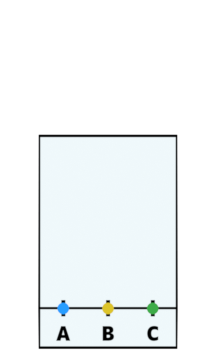
\includegraphics[height=0.2\textheight]{images/chimie/CCM/CCM_protocole0003.png} \\      
      À l'aide d'un cure-dent, déposer chaque échantillon sur un emplacement bien délimité.
    \end{center}
  \end{multicols}
  
  \bigskip
  
  \begin{multicols}{2}
    \begin{center}
      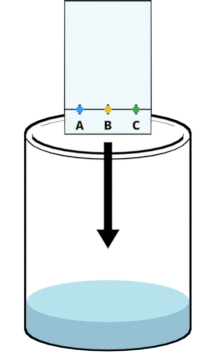
\includegraphics[height=0.2\textheight]{images/chimie/CCM/CCM_protocole0004.png}
      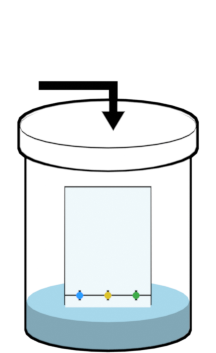
\includegraphics[height=0.2\textheight]{images/chimie/CCM/CCM_protocole0005.png} \\      
      Poser doucement la plaque dans la cuve en la tenant par les côtés et fermer la cuve.
      \important{Il ne faut jamais déplacer la cuve} et attendre que l'éluant monte.
    \end{center}

    \begin{center}
      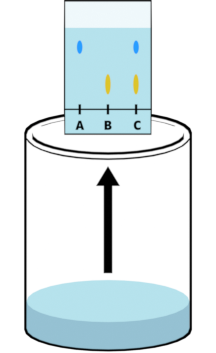
\includegraphics[height=0.2\textheight]{images/chimie/CCM/CCM_protocole0006.png} \\      
      Quand le front de l'éluant s'approche du haut, sortir la plaque.
      Tracer une ligne indiquant la hauteur où l'éluant est monté.
    \end{center}
  \end{multicols}
\end{doc}


%%%% questions
\mesure
Placer un M\&M's dans chaque tube à essais et les recouvrir d'eau.
Attendre que le colorant se soit dissous dans l'eau et récupérer les M\&M's.

\mesure
Réaliser le protocole du document~\ref{doc:TP4_protocole_CCM}, avec un dépôt de colorant jaune, un dépôt de colorant bleu et deux dépôts des solutions préparées précédemment.

\mesure
Schématiser le chromatogramme obtenu, en indiquant clairement les différentes tâches, la ligne de dépôt et le front de l'éluant.
\pasCorrection{\vfill}

\question{
  Pourquoi doit-on placer la ligne de dépôt au dessus du niveau de l'éluant ?
}{
  Si on la place en dessous, le dépôt va se diluer dans l'éluant et ne montera pas sur la plaque.
}[2]

\question{
  Pourquoi ne doit-on pas déplacer la cuve pendant la montée de l'éluant ?
}{
  Si on déplace la cuve, l'éluant va monter de manière irrégulière, ce qui va fausser l'analyse des résultats.
}[2]


%%%%
\pasCorrection{\newpage}
\begin{doc}{Lecture d'un chromatogramme}{doc:TP4_lecture_chromato}
  \separationBlocs{
    \begin{listePoints}
      \item \important{Lecture verticale :} si le dépôt d'un échantillon se sépare en plusieurs tâches, il s'agit d'un mélange. 
      Le nombre de tâches indique le nombre d'espèces chimiques qui composent le mélange.
      \item \important{Lecture horizontale :} sur une même plaque, une même espèce chimique migre toujours à la même hauteur. 
      Et donc si deux tâches sont à \important{la même hauteur, alors elles sont la même espèce chimique.}
    \end{listePoints}
    \vfill \strut
  }{
    \centering
    \vspace*{-20pt}
    \image{0.8}{images/chimie/CCM/chromatogramme.png} \\
    \legende{schéma d'un chromatogramme}
  }
\end{doc}

%%%%
\begin{doc}{Colorants alimentaires}{doc:TP4_colorants_alimentaire}
  \begin{listePoints}
    \item \important{E102 : jaune de tartrazine.} Son usage doit s'accompagner en France de la mention « peut avoir des effets indésirables sur l'activité et l'attention chez les enfants ».
    \item \important{E133 : bleu brillant.} Un enfant de 40 kg peut ingérer jusqu'à \qty{240}{\mg} de bleu brillant en une journée. Au-delà le conseil européen indique que ce produit peut être toxique.
  \end{listePoints}
\end{doc}

\question{
  En analysant le chromatogramme à l'aide du document~\ref{doc:TP4_lecture_chromato}, indiquer si les échantillons sont des corps purs ou des mélanges.
}{
  Pour le bleu et le jaune, on a des corps purs (une seule tâche).
  Pour le vert on a un mélange, car le dépôt s'est séparé en deux tâches.
}[5]

\question{
  En utilisant le chromatogramme, donner la composition des colorants présents sur la couche externe des M\&M's.
}{
  Le jaune et le bleu du M\&M's montent à la même hauteurs que les dépots de colorant jaune E102 et bleu E133, ce sont donc les mêmes espèces chimiques.
}[5]


\pasCorrection{\newpage}

\important{\large Composition des huiles essentielle d'orange et de citron}

%%%% Contexte
\begin{contexte}
  Les huiles essentielles sont obtenues à partir de végétaux pressés ou par distillation fractionnée.
  Les huiles essentielles sont riches en molécules odorantes.
  
  \problematique{
    Comment décrire la composition d'une huile essentielle à l'aide d'une CCM ?
  }
\end{contexte}


%%%% docs
\separationBlocs{
  %%
  \begin{doc}{Huile essentielle de citron et d'orange}{doc:TP4_huile_essentielle}
    L'huile essentielle d'orange (HEO) et l'huile essentielle de citron (HEC)
    sont obtenues en pressant les zestes d'une orange et d'un citron respectivement.
  \end{doc}
}[0.31]{
  %%
  \begin{doc}{Odorat et molécules odorantes}{doc:TP4_molecules_odorantes}
    Chez les humains, Les molécules odorantes sont captées par des neurones de l’épithélium olfactif,
    puis ces neurones transmettent l'information nerveuse au cerveau qui y associe une odeur.
  
    Voilà quelques exemples de molécules odorantes :
    \begin{listePoints}
      \item le \important{limonène} (Lim), est associé à une odeur d'orange.
      \item le \important{linalol} (Lin), est associé à une odeur fraiche et florale.
      \item le \important{géraniol} (G), est associé à une odeur de rose.
      \item le \important{citral} (Ci), est associé à une odeur de citron.
    \end{listePoints}
  \end{doc}
}[0.69]


%%%%
\question{
  Quelles molécules odorantes peut-on trouver dans l'huile essentiel de citron et d'orange ?
}{
  D'après les descriptions du document~\ref{doc:TP4_molecules_odorantes},
  on s'attend à trouver du limonène dans l'huile essentielle d'orange et du citral dans l'huile essentielle de citron.
}[2]

\begin{doc}{Résultat d'une CCM}{doc:TP4_HEC_HEO}
  On a réalisé deux CCM pour déterminer la composition des huiles essentielles d'orange et de citron.
  \begin{center}
    \image{0.25}{images/donnees/chromato_HEC}
    \image{0.25}{images/donnees/chromato_HEO}
  \end{center}
\end{doc}

\question{
  En analysant les chromatogrammes, donner la composition des huiles essentielles de citron et d'orange (HEC et HEO).
}{
  On trouve du limonène, du géraniol et du citral dans l'HEC (tâches à la même hauteur).
  On trouve du limonène et du géraniol dans l'HEO.
}[5]
